%\chapter{cap}
\chapter{Calculos Básicos}
\label{cap:calculos}
Parametros para calculos
Fator de potência indica quando a energia solicitada da rede está sendo usada de forma útil. \textbf{$FP= cos \phi < 1,0$}
Tipos de linhas método de referência para a capacidade de corrente, \textbf{B1} que equivale a cabos isolados em eletrodutos circulares embutidos ou aparentes, o modo mais comun de instalação considerado até a entrada do quadro.
Do quadro até os gabinetes \textbf{ B2} cabos multipolares.
Numero de condutores carregados, considerando 2 para monofásicos e 3 para trifásicos.
Cabos de cobre 70ºC isolação PVC


\section{Corrente de projeto Ip ou Ib}
Corrente de projeto ($I_{p}$) ou ($I_{b})$ que os condutores devem suportar levando em consideração suas características nominais (Tabela \ref{tab:eqIp}).

\begin{table}[htbp]
\caption{Equações utilizadas para encontrar a corrente nominal de projeto.}
\begin{center}
\begin{tabular}{|c|c|}
\hline
Circuito & Equação \\ \hline
Monofásico (F+N) &\rule{0pt}{12pt} $I_{p}=\frac{P_{n}}{V \cdot \cos \varphi \cdot \eta}$ \rule[-6pt]{0pt}{0pt} \\ \hline
Trifásico (3F+N) & \rule{0pt}{12pt} $I_{p}=\frac{P_{n}}{\sqrt{3} \cdot V \cdot \cos \varphi \cdot \eta}$ \rule[-6pt]{0pt}{0pt} \\ \hline
\end{tabular}
\label{tab:eqIp}
\end{center}
\end{table}
%\begin{table}[htbp]
%\caption{Equações utilizadas para encontrar a corrente nominal de projeto.}
%\begin{tabular}{|c|c|}
%\hline
%Circuito & Equação \\ \hline
%Monofáscio (F+N) & \begin{equation}
%I_{p}=P_{n} over {V cdot cos %varphi cdot %eta}
%\end{equation} \\ \hline
%trifásico (3F+N) & 
%\begin{equation}
%I_{p}=P_{n} over { sqrt{3} cdot V CDOT cos %varphi  cdot %eta}
%\end{equation} \\ \hline
%\end{tabular}
%\label{tab:eqIp}
%\end{table}

%tabela
%Circuito
%Formula
%Monofásico (F + N)
%
%Trifásico (3F + N)
%tabela com formula
%Sendo:
%\begin{equation}
%
%I_{p} = I_{p}  leslant I_{n} leslant I_{z} ; (b) I_{2} leslant 1,45 cdot I_{z}
%
%\end{equation}

%\begin{equation}
%I_{p}=P_{n} over { sqrt{3} cdot V CDOT cos %varphi  cdot %eta}
%\end{equation}


Esquema de distribuição de condutores vivos:
Corrente alternada monofásico a dois condutores F + N (220V ou 127V)
Corrente alternada trifásico a quatro condutores 3F + N (380V ou 220V)

\section{Metodos para dimensionamento de cabos}

 Método de referência para os calculos de capacidade de condução de corrente
B1
Condutores isolados ou cabos unipolares em eletroduto circulares aparaente ou embutido em alvenaria. Tipo de instalação mais comum, considerado para alimentação do QDP (quadro de distribuição do painel).
Esquema de aterramento
A alimentação do quadro de ser composto por uma proteção PE (aterramento), um neutro,  uma fase para monofásica ou três fases para trifásica
Em esquema TN o seccionaento automático visando proteção contra choque elétrico, pode ser usados dispositivos de proteção de sobrecorrente, dispositivos de proteção a corrente diferencial-residual (dispositivo DR), sendo este não é admitido quando usando a variante TN-C.


Pn – Potência elétrica nominal (W);
V – Tensão elétrica entre fase (V);
$\eta$ – Rendimento considerado = 1;
cos $\varpi$ -  fator de potência (considerado = 1)
Numero de condutores carregados:
    • 2 para alimentação de quadro monofásico e circuitos de distribuição;
    • 3 para alimentação de quadro trifásico.
Tabela 2: Capacidade de condução de corrente (A) para metodo B1; condutor de cobre, 70°C, PVC, temperatura ambiente 30°C(ar). Fonte tabela 36 NBR 5410:2004
começo tabela
fim tabela

    Parâmentros de projeto
        Corrente de curto circuito:   A
        Queda de tensão
        Fatores de demanda considerados
        Temperatura ambiente
    • Cálculo de demanda
    • Dimensionamento dos condutores
    • Dimensionamento dos eletrodutos
    • Dimensionamento das proteções
\subsection{ Metodo da queda de tensão}
Para a alimentaçao principal a distancia L dentro do quadro 1,2 m no pior caso Quadro 10x3.  Para alimentação da tomada = 0,95 m. Para os Circuitos L = 5 m


\subsection{Dimensionamento Neutro e PE}

\begin{description}
\item[Circuito monofásico] Neutro com mesma seção do condutor de fase.
\item[Circuito trifásico com taxa de terceira harmônica e seus multiplos inferior que  33\%]  Neutro com mesma seção dos condutores de fase.
\end{description}
Para circuitos trifásicos equilibrados, com taxa de 3ª Harmonica menor que 15\%, ou condutor neutro protegido contra sobrecorrente, conforme tabela 48 da NBR 5410:2004, até a seção de Fase menor ou igual 25 mm², seção dos condutores de  neutro tem mesma seção. Para seção fase 35 mm², seção Neutro 25 mm². 

Para condutores de proteção equipotencia PE é a mesma que condutor fase no mesmo conduto até 16 mm². Para fase 25 mm² e 35 mm², PE 16 mm². 


\subsection{ Metodo de instalação}

Dimensionamento de condutos
\section{ Proteção}
O quadro de ditribuição contém os dispotivos de proteção, ele que vai receber os condutores de alimentação que vem do quadro geral. E é dele que partem os circuitos para alimentação dos grupos de modulo do painel. 
%Vamos chama-lo de QT _ X _ _ P_ ___V



\subsection{Proteção contra Sobrecorrente (Sobrecarga e curto-circuito)}


Dispostivos de proteção deve interromper toda corrente de sobrecarga nos condutores dos circuitos antes que ela possa provocar aquecimento que prejudique a isolação, terminais ou vizinhanças das linha. Para esta proteção deve ser assegurada a coordenação entre o dispotivo de proteção e os condutores, satisfazendo as seguintes condições.
\begin{enumerate}
\item \begin{equation}
		I_{b} \leq I_{n} (ou I_{c}) \leq I_{z};
		\end{equation}
\item \begin{equation}
		I_{2} \leq I_{n} \leq I_{z}(ou I_{c});
		\end{equation}
\end{enumerate}

Sendo:
$I_{b}$ – corrente de projeto (A)
$I_{n}$ – corrente nominal do dispositivo de proteção (A)
$I_{c}$ -Capacidade de condução de corrente dos condutores vivos do circuito nas condições de instalação.
$I_{z}$ –  Ic submetido a fatores de correção de agrupamento e ou fatores de correção de temperatura.
$I_{2}$ – Corrente de atuação do dispositivo de proteção.

Portanto, as correntes caracteristicas dos conjunto condutor-disjuntor devem atender as condições (Figura \ref{fig:disjatu}):
\begin{itemize}
\item Para evitar a atuação do disjuntor quando o circuito estiver em condição normal de funcionamento: a corrente nominal do disjuntor ($I_{n}$), não deve ser menor que a corrente de projeto ($I_{b}$).
\item Para que o disjuntor perceba a ocorrência de sobrecarga no circuito: a corrente nominal do disjuntor ($I_{n}$), não deve ser maior que a capacidade de condução de corrente ($I_{z}$) dos condutores.
\item A capacidade de condução de corrente ($I_{z}$) dos condutores devem ser maior que a corrente de projeto ($I_{b}$)

\end{itemize}

acrescetar uma foto do disjuntor representando as grandezas das correntes
\begin{figure}[ht]
    \centering
    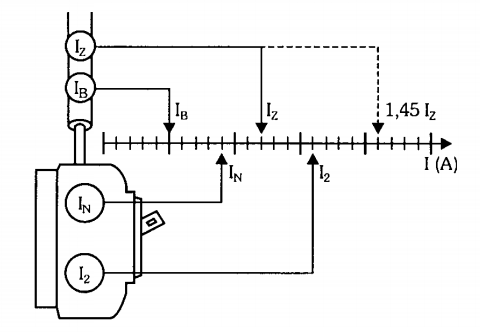
\includegraphics{image/disjAtua.png}
  %  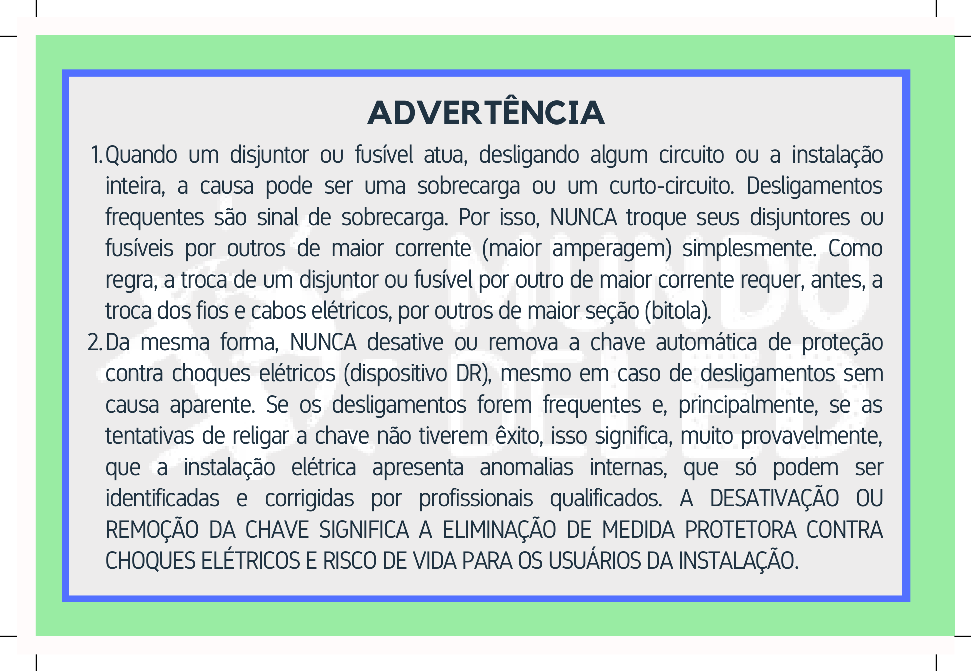
\includegraphics[scale=0.5]{image/EtiqAdvQD.pdf}
    \caption{Representação das condições de atuação contra sobrecarga (NBR 5410:2004 item 5.3.4)}
    \label{fig:disjatu}
\end{figure}

\subsubsection{ Disjuntores dimensionamento}

		METODO DE CALCULO DE CURTO-CIRCUITO
		Coordenação e seletividade de disjuntores
\subsection{ Contra choques elétricos }
	6.1.2.1 Esquemas de aterramento
	6.1.2.2 IDR dimensionamento

\subsection{ Proteção contra sobretensões}

\subsection{ Contra descarga atmosférica}

	Compatibilidade eletromagnética
\subsection{Quadros e acessórios}

    • Quadro de distribuição
        ◦ diagrama esquemático unifilar
        ◦ diagrama esquemático multifilar
    • Especificações dos componentes
    • Lista de materiais
Avisos devem ser colocados no quadro
foto do adesivo
Colocar aqui os adesivos e criar um anexo para a impressão dos adesivos.
Colocar os tamanhos de quadro metalicos disponiveis, considerados
ATENÇÃO A MANUTENÇÃO DO QUADRO ELETRICO DEVE SER REALIZADO POR PESSOAL HABILITADO. RISCO DE CHOQUE.

\subsection{Bornes}
 
Os bornes as serem escolhidos devem ser preparados para a fixação em trilho DIN 35mm. Neste projeto a sugestão é utilizar os bornes de passagem padrão compativeis com os cabos e a corrente. Na Tabela \ref{tab:bornes} tem a capacidade de corrente para cada borne e sua seção de condutores máxima. 
Os bornes de passagem servirão para as entradas e saídas de fase e neutro. Para melhor sinalização usar borne azul para o condutores de neutro.
O borne de proteção equipotencial (aterramento) tem cor verde-amarela, deve ser escolhido pela seção dos conectores. ATENÇÃO NUNCA UTILIZAR BORNES VERDE-AMARELO para conexão de fase ou neutro.
Poste final são usados para fixar os bornes para que não corra no trilho.
Plaquetas separadoras podem ser usadas para separar grupos de bornes, porém deve ser utilizada nos caso onde haja a necessidade de isolar a parte condutora exposta.

\begin{table}[htbp]
\caption{Bornes tem capacidade tensão de 8OO VCA. Nesta tabela tem capacidade de corrente considerando a seção de cabos, da linha Bornes ALPHA FIX da Siemens com conexão por parafuso}
\begin{tabular}{|l|l|l|l|l|l|l|}
\hline
Tipo & cor & 2,5 mm² & 4 mm² & 6 mm² & 16 mm² & 35 mm² \\ \hline
Borne Padrão & bege, azul, laranja & 24 A & 32 A & 41 A & 76 A & 125 A \\ \hline
\end{tabular}
\label{tab:bornes}
\end{table}


\subsection{Etiquetas}

Conforme \cite{NBRIEC61439-12017} 
\begin{quote}
O montador do CONJUNTO deve prover para cada CONJUNTO uma ou mais etiquetas, marcadas de uma maneira durável e dispostas em um local onde estejam visíveis e legíveis quando o CONJUNTO estiver instalado e em funcionamento.
\end{quote}
As informações devem ser:
\begin{enumerate}
\item o nome do montador ou marca comercial (3.10.2)
\item designação do tipo ou numero de identificação ou meio que torne possivel obter do montador do CONJUNTO  as informações apropriadas.
\item data de fabricação
\item identificação da ABNT NBR IEC 61439-X (parte especifica "X" deve ser identificada)
\end{enumerate}

Deve ser fornecido documentos ou catálogos as condições de manuseio, instalação, funcionaento e manutenção do CONJUNTO e os equipamentos nele contido.

Deve ser disponibilizado instruções sobre peso e medidas para o transporte, o manuseio, a instalação e o funcionamento do CONJUTO sejam corretos e apropriados. 

Indicar a manutenção e sua periocidadede recomendada.


\begin{figure}[ht]
    \centering
    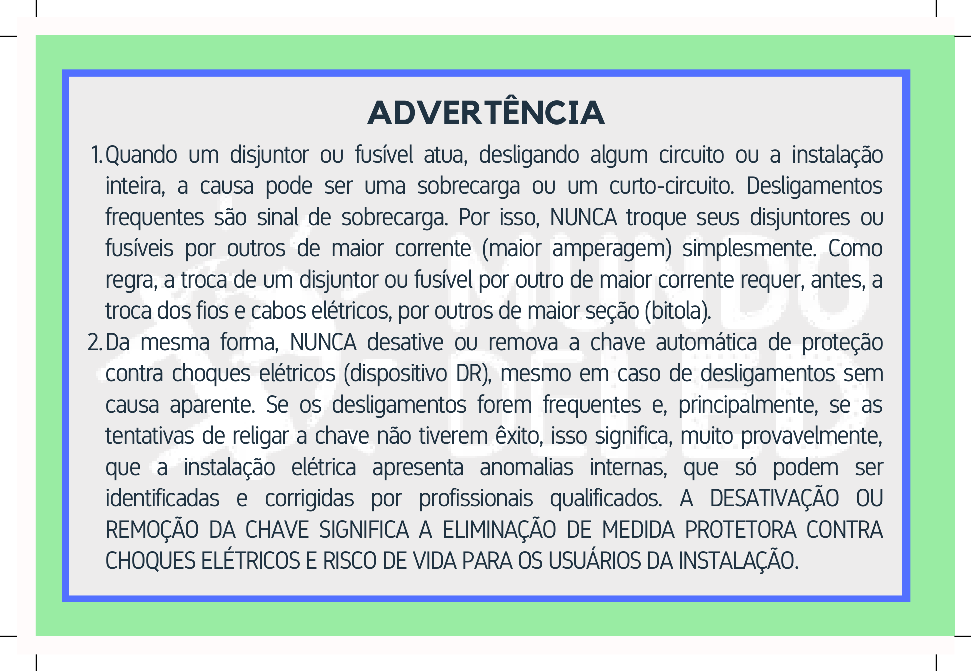
\includegraphics{image/EtiqAdvQD.pdf}
  %  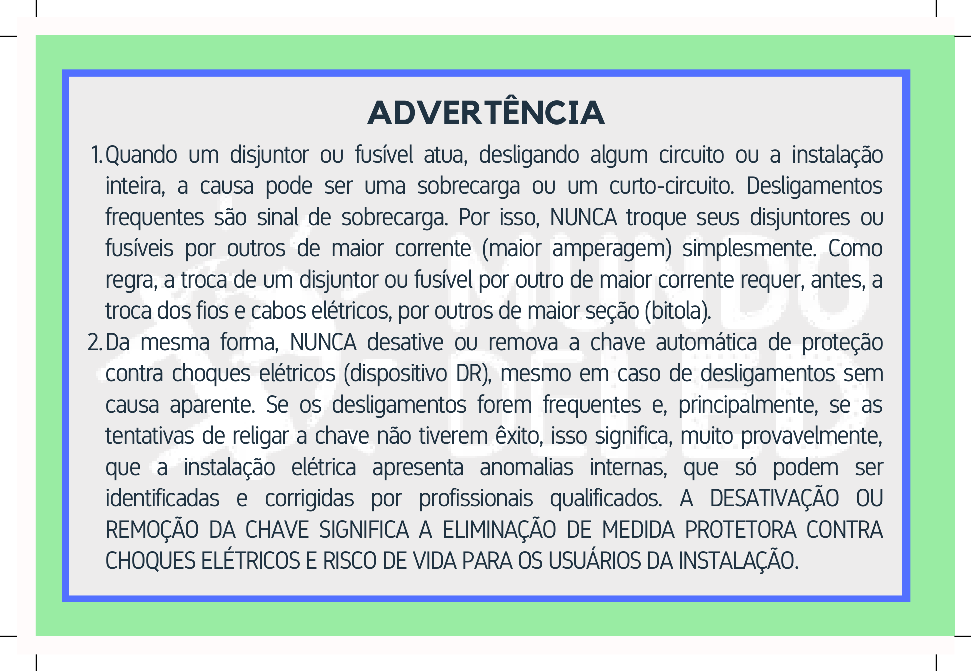
\includegraphics[scale=0.5]{image/EtiqAdvQD.pdf}
    \caption{Legenda da imagem}
    \label{fig:etiqueta}
\end{figure}

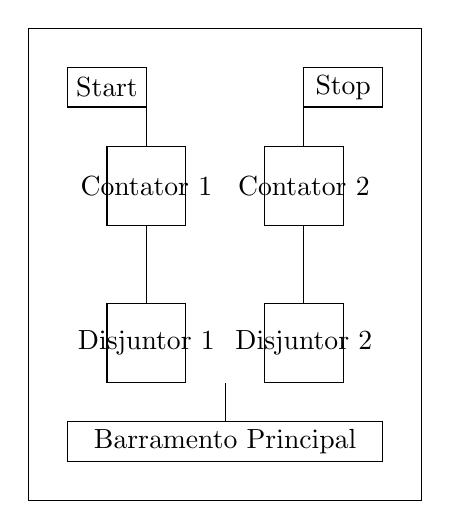
\begin{tikzpicture}[scale=0.5]
    % Caixa do quadro
    \draw (0,0) rectangle (10,12);
    % Barramento principal
    \draw (1,1) rectangle (9,2);
    \node at (5,1.5) {Barramento Principal};
    % Disjuntores
    \draw (2,3) rectangle (4,5);
    \node at (3,4) {Disjuntor 1};
    \draw (6,3) rectangle (8,5);
    \node at (7,4) {Disjuntor 2};
    % Contatores
    \draw (2,7) rectangle (4,9);
    \node at (3,8) {Contator 1};
    \draw (6,7) rectangle (8,9);
    \node at (7,8) {Contator 2};
    % Botões de comando
    \draw (1,10) rectangle (3,11);
    \node at (2,10.5) {Start};
    \draw (7,10) rectangle (9,11);
    \node at (8,10.5) {Stop};
    % Fiação
    \draw (5,2) -- (5,3);
    \draw (3,5) -- (3,7) -- (2,7);
    \draw (7,5) -- (7,7) -- (8,7);
    \draw (3,9) -- (3,11) -- (1,11);
    \draw (7,9) -- (7,11) -- (9,11);
\end{tikzpicture}

\section{Problemas e soluções}
Problema: Disparos dos dispositivos de proteção podem ser gerados pelas correntes de pico gerado ao ligar o painel. 
Solução: Escolher disjuntores com curva de disparo menos sensivel, por exemplo alterando da curva C para a curva D. 
Inicializar os circuitos sucessivamente, utilizando temporizadores auxiliares em relés de controle.\textbf{Não deve trocar o disjuntor por outro de maior capacidade pois isto pode tornar as conexões eletricas sem proteção}
